\documentclass[a4paper,10pt]{article}
\usepackage[utf8]{inputenc}
\usepackage[T1]{fontenc}
\usepackage[english]{babel}
\usepackage[a4paper]{geometry}
\usepackage{graphicx}
\usepackage{float}


\title{Software Architectures\\ Assignment 5 : Software Visualizations}
\author{Arnaud Rosette, Simon Picard}
\date{May 21 2015}

\begin{document}
\maketitle
\section{Exercise 1 : Analyzing the web portal application with an existing visualization}
\subsection{Chosen visualization}
As required by the assignment, we chose a predefined visualization of Moose. We decided to use the Blueprint complexity visualization because it highlights the complexity of a class, the cohesion inside a class, the coupling between different classes and the class hierarchy. So this visualization is able to show us the application architecture from a close perspective as well as a large perspective.
\begin{figure}[H]
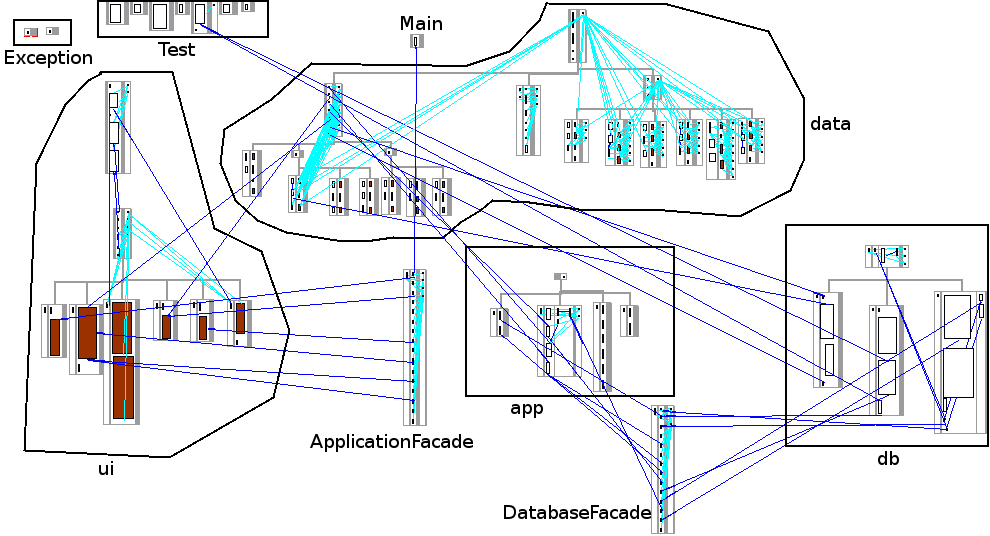
\includegraphics[width=\textwidth]{src/blueprint.png}
\centering
\caption{Class hierarchy Blueprint of the web\_portal application}
\end{figure}
\subsection{Lonely classes}
The visualization shows several classes that are isolated from the rest of application. They are classes which handle exceptions or classes managing test cases.\\
As we can see, the exception classes are only composed of one constructor. The coupling is very low between these classes and the rest of the application because the only thing that the other classes know about these classes is their constructor. It is a rather regular behavior for exception classes.\\
Most of test classes are essentially composed of one small  main method. It indicates that the test cases are poor in this application. Each test class only interacts with the class it needs to test. For example, TestRegularDatabase only interacts with RegularDatabase. It highlights the fact that the function of each test class is well defined. Some of the invocations are missing in this visualization for several test classes because each test class call at least one method of the class that it test.

\subsection{3-tier architecture}
The Blueprint visualization highlights the fact that the application is based on a layered architecture (3-tier architecture). We can see that each layer (ui, app and db) only interacts with the sub-layer through a facade. So the interface between each layer is clearly defined. We can notice that some invocations are missing from the ApplicationFacade to the app package.\\
The figure also shows that the two facades interact with concrete classes. The ApplicationFacade class uses concrete classes of the app package and DatabaseFacade uses concrete classes of the db package. DatabaseFacade interacts with the current implementation of the database layer which is a sql database. So coupling between different layers is rather low but coupling between a facade and classes inside the same package is quite high because facade uses directly concrete implementation. In order to address this issue, facades have to be independent from their layer implementation which means that facades have to talk to abstract classes instead of talking to concrete classes.

\subsection{Cohesion}
The graph exhibits a quite high cohesion inside classes. Indeed, most of the accesses are realized inside a class or between a sub-class and its parent class. The rest of the interactions between classes are invocations and their number is lower than that of accesses.

\subsection{Coupling}
The coupling between classes is relatively low thanks to the layered architecture but it can be improved because the coupling inside a package can be lower, especially between a facade and the classes in the same package. Facade classes have to interact with abstract classes in order to be able to switch from an implementation to another with few modifications in the facade class.

\section{Exercise 2 : Building our own visualization with Mondrian}
\subsection{Created visualisation}
The newly created visualisation shows the classes and their methods, the classes are linked in light grey to their parents and their children. Each methods of the class is a square either green or red, if it is green it means that the method contains comments, red otherwise. There are some other links, they are blue arrow, linking the class to the class that test them.\\
The metrics are :
\begin{itemize}
\item Number of class
\item Class inheritance
\item Number of methods per class
\item Presence of comments
\item Presence of tests
\end{itemize}

Those metrics focus on the code quality of the program because the blueprint already shows many aspects of the architecture including classes interaction. In the following subsections, each metrics will be analysed for this project with an explaination of why they are important.
\begin{figure}[h]
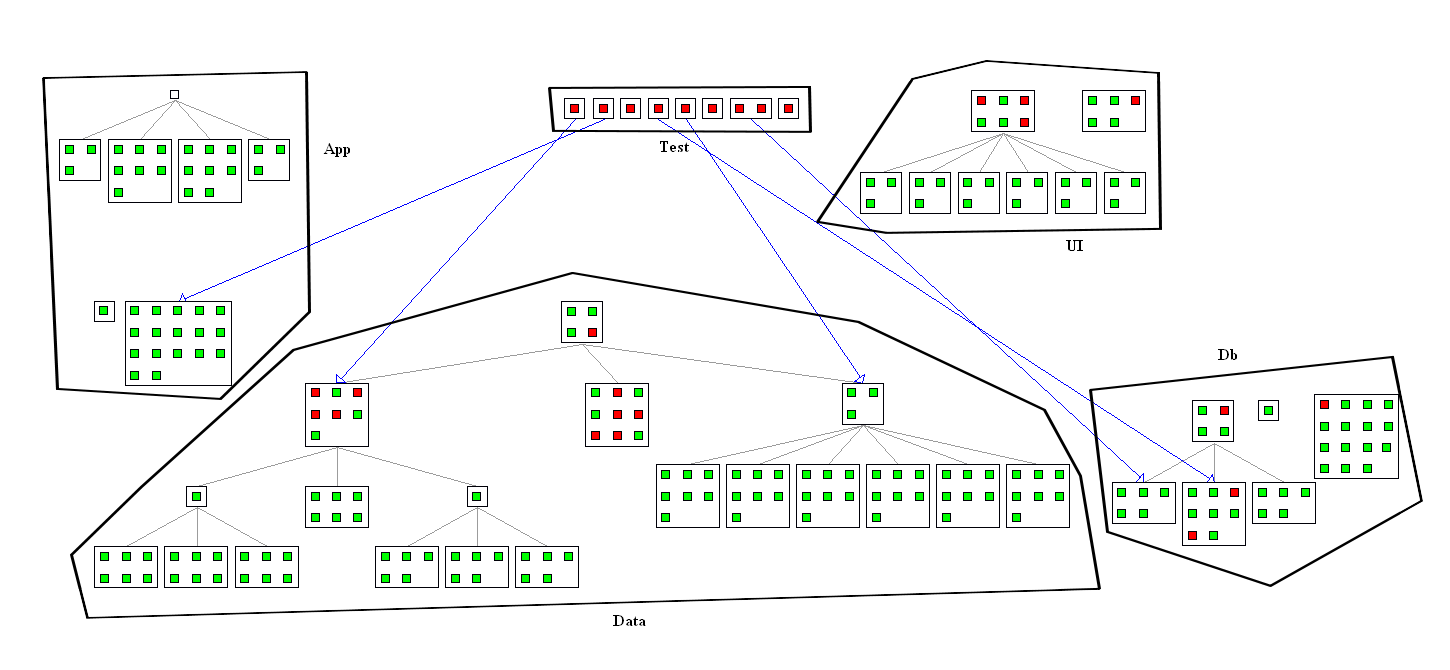
\includegraphics[width=\textwidth]{src/tc2.png}
\caption{A representation of the web\_portal service showing comments and test}
\end{figure}
\subsection{Comments}
In the visualisation, we can observe that there is a majority of green methods, meaning that they are commented. Nevertheless their is still some red methods, i.e without comments. Majority of red methods are in mono method classes, those are either exceptions or tests. The methods should always be commented, indeed it offers an easier comprehension in further developing but, in extrem programming the comments are forbiden, the code should be readable by itself by using adequate variable name.

\subsection{Tests}
The representation shows a really poor test use. Indeed, only five tests are printed and most of the time there is only one method so we can assume that only few functionnalities are tested. The tests are the main tool for the developper, in some agile methods, the tests are created even before the functionnalities itself. The tests are important because they can help in assuring that everything works, and if they are good, the diffuculties in adding new functionnalities to the existing ones show up directly. Adding revelant tests might be the first improvement to do in this project.\\
Note: some test classes are not linked, the matching test between two classes is done by comparing the name of them so some test dependance might be miss.

\subsection{Methods}
In this visualisation, we can observe the methods of the classes. If we focus on the one with the same number of methods and inheriting from the same class, one could ask himself if it would not be a good idea to refactor his architecture by adding some more inheritance. In the project, the structure of the datas are close, by example, RegularData inherit from Data but some child of RegularData could be regrouped by abstract classes.

\subsection{Code}
\begin{verbatim}

| view classes edges tests edges2|
classes := MooseModel root allModels first allModelClasses.
view := MOViewRenderer new.
edges := OrderedCollection new.
edges2 := OrderedCollection new.
tests := classes select: [:c | c name beginsWith: 'Test'].

view nodes: classes forEach: [ :class |
        view shape rectangle withoutBorder.
        (tests select: [:c | c name = ('Test', class name)]) do: [:t | edges add: t->class ].
        view nodes: class methods forEach: [ :method | 
                view shape rectangle 
                fillColor: [method hasComments ifTrue: Color green ifFalse: Color red];
                width: 5;
                height: 5.
            view node: method. 
            view gridLayout gapSize: 2.
        ].
        view gridLayout gapSize: 1.].
edges2 := view edgesFrom: #superclass.
view shape arrowedLine color: Color blue.
view edges: edges from: #key to: #value.

view treeLayout userDefinedEdges: edges2.
view open.
\end{verbatim}
\end{document}
